\section{Übung 3 - Eigenkapital}

\textbf{Bewertung von Aktien}:
\begin{itemize}
	\item \textbf{Dividend-Discount Modell}: $\text{Aktienpreis}=\frac{D_1}{(1+k_E)}+\frac{D_2}{(1+k_E)^2}+\ldots+\frac{D_t}{(1+k_E)^t}+\ldots$ mit $D_i$: Dividende in Periode $i$, $k_E$: Eigenkapitalkosten
	\item \textbf{Constant-Dividend-Growth Modell}: Jährliche Dividende nimmt mit der gleichen konstanten Wachstumsrate $g$ zu
	$$\text{Aktienpreis}=\frac{D_0(1+g)}{k_E-g}$$
	\item \textbf{Multi-Stage Dividend-Growth Modell}: Dividende $D_0$ wächst mit einer über-durchschnittlichen jährlichen Wachstumsrate $g_1$ für $T$ Jahre. Ab Jahr $T+1$ wächst die Dividende bis in die Ewigkeit mit einer geringeren Wachstumsrate $g_2$
	\item \textbf{Discounted-Cash-Flow-Bewertung}: Gesamtwert eines Unternehmens entspricht Summe aus EK und Netto-FK und entspricht den diskontierten Free Cash Flows des Unternehmens 
\end{itemize}
\bigskip
\textbf{Erwartete Rendite} = Erwarteter Gewinn / Investition

\textbf{Signaling Theory}: Zur Reduktion des Underpricings dienen Indikatoren als Signale für Investoren
\begin{center}
	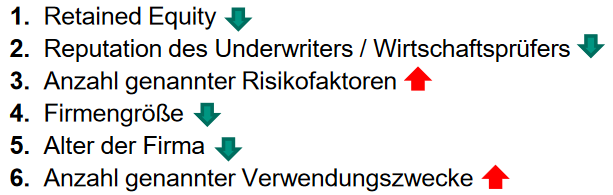
\includegraphics[width=0.5\textwidth]{images/e6.png}
\end{center}